%!TEX root = ../dissertation.tex
\chapter{Experiments}

\section{Symmetry-aware Map Optimization}
As one of our two main data structures, the memory usage of our symmetry-aware map is something that was very important to us.
We found that we often had trouble running large data sets because we would run out of memory before certifying the optimal rule list.
In these long runs, our permutation map would grow to be hundreds of thousands or millions of entries large.
Thus, carrying a lot of memory overhead with each node led to serious memory bloat and ran us out of memory.
This section explores some of the techniques we used to handle this memory bloat.

Our symmetry-aware map was originally an STL map with keys as STL sets of size\_t and values as pairs of STL vectors of size\_t and a double.
The first problem is that the STL map is implemented as a red-black tree, meaning every node had the overhead of multiple pointers pointing to its children.
This can be solved using a STL unordered map, which is implemented as a hashtable.
That has some overhead, since it will allocate more buckets than are filled, but nowhere near to the two pointers per node of overhead of the STL map.

Next, the representation of the rule ids no longer had to be size\_t.
We made an assumption that we'll never have more than 65000 rules, so we used unsigned shorts for our rule ids.
This means that our final data structure was able to use only 2 bytes per rule id instead of 8 bytes for a size\_t.
Since we're keeping two different representations of the prefix--the canonical order and the actual order of the prefix, and these prefixes can be of length on the order of 5 rules, saving 6 bytes per rule translates to a lot of 

Our initial implementation used an STL set as the key, which carries a lot of overhead because of all the operations that a set needs to support.
For a prefix of length 6, the corresponding key therefore takes up 
After starting with the STL set, we transition to a sorted STL vector.
This reduced overhead because a vector is essentially just an array with a little bit of overhead.
However, all of these STL containers support a broader range of operations than we needed.
All we needed was some way to compare the canonical orders and determine if they were the same.
We eventually achieved this simply by allocating a chunk of memory that held the length of the prefix and the sorted order of the ids.
This means that, for a prefix of length 6, we use 14 bytes for the key.

We had a similar set of issues with our values for the permutation map.
Beginning with a STL vector to keep track of the actual order of the rules in the prefix, we again wanted to remove the overhead incurred by the fact that STL containers need to support a wider array of operations than we needed.
Thus, we could use a similar technique to what we did with the keys to keep track of the prefix order.
However, in fact, we can do even better because we already have a canonical representation of the rules--all we need in the value was the ordering of those rules.
Thus, we can use unsigned chars instead of unsigned shorts to record the index of where the rules in the canonical order are in the prefix.

However, these optimizations all pertained to the symmetry-aware map with prefix keys.
Dealing with the captured vector keys required a different approach.
Our captured vectors were of type mpz, and since unordered\_map requires a custom hash for unsupported types, we had to find a way around that.
STL has some hash functions for built in types, so we initially wrote a function to convert between our VECTOR type and a $std::vector<bool>$.
This conversion turned out to be very slow, especially as we were running on data sets with many samples, meaning these mpz types were fairly memory intensive.
Once we wrote our own hash function and were able to use our mpz type again, it became much faster.

\section{Ablation--how much does each bound/optimization help?}

We ran a number of experiments where we only took out one component and measured the effects on the time and memory of our algorithm.
We find that each optimization and bound is extremely important to concluding the algorithm quickly and in a reasonable amount of memory.
These were all executed on a MacBook Air with 8GB of RAM.

\subsection{Full CORELS system}

Running the full CORELS system on the COMPAS dataset yields the optimal solution and its certificate within 121s.

\begin{figure}[t!]
\begin{center}
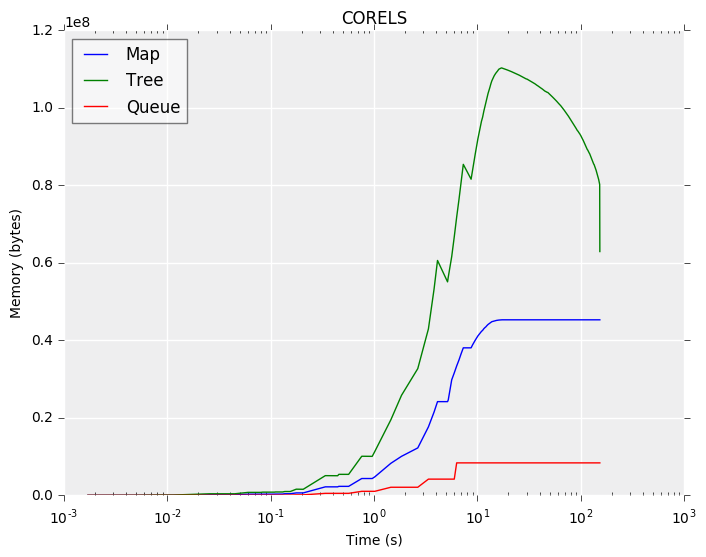
\includegraphics[width=0.4\textwidth]{figs/corels_mem.png}
\end{center}
\caption{}
\label{fig:prefix-captured}
\end{figure}

\subsection{Priority Queue} \label{exp:priority}
142.s

\subsecton{Support Bounds}
261s

\subsection{Symmetry-aware map}

\subsection{Lookahead Bound}

\subsection{Equivalent points bound}

\subsection{Objective Bound}

\section{Parallelization}
The tree structure of our trie lends itself nicely to parallelization.

We began by trying to parallelize the inner loop of our incremental evaluation.
This 
This had too much contention.

Instead, we can parallelize the search over the tree itself.